%*****************************************
\chapter{Implementation}
\label{ch:implementation}
%*****************************************

\hint{This chapter should describe the details of the implementation addressing the following questions: \\ \\
1. What are the design decisions made? \\
2. What is the environment the approach is developed in? \\
3. How are components mapped to classes of the source code? \\
4. How do the components interact with each other?  \\
5. What are limitations of the implementation? \\ \\
The section should have a length of about five pages.}
\section{Design Decisions}
\textbf{Tensorflow 2.0} is used as the framework for all experiments presented in this thesis. It enables software development on a high level of abstraction while ensuring code performance. Because some
procedures are not naturally compatible with the implementation of Tensorflow 2.0  this thesis needs to employ a few workarounds. Notably pruned weights are not removed from the network but rather set to zero each time a layer is evaluated. As such they do not affect the predictions but are influenced by backpropagation. \textit{The effect on the presented experiments is unclear to me.}

\subsection{Missing Parameters}
Through the related work referenced in this thesis specifications of any one model where incomplete. The following subsection aims to explain how the parameters were inferred or chosen. 
\begin{itemize}
	\item Activation function for most layers
	\item Activation function for output layers
	\item Dropout rate
	\item padding in CNNs
	\item ...
\end{itemize}

\section{Architecture}
\begin{figure}[H]
	\centering
	\includegraphics[width=450px]{gfx/structure.png}
	\caption{project architecture}
	\label{fig:Architecture}
\end{figure}

\section{Interaction of Components}
\begin{figure}[H]
	\centering
	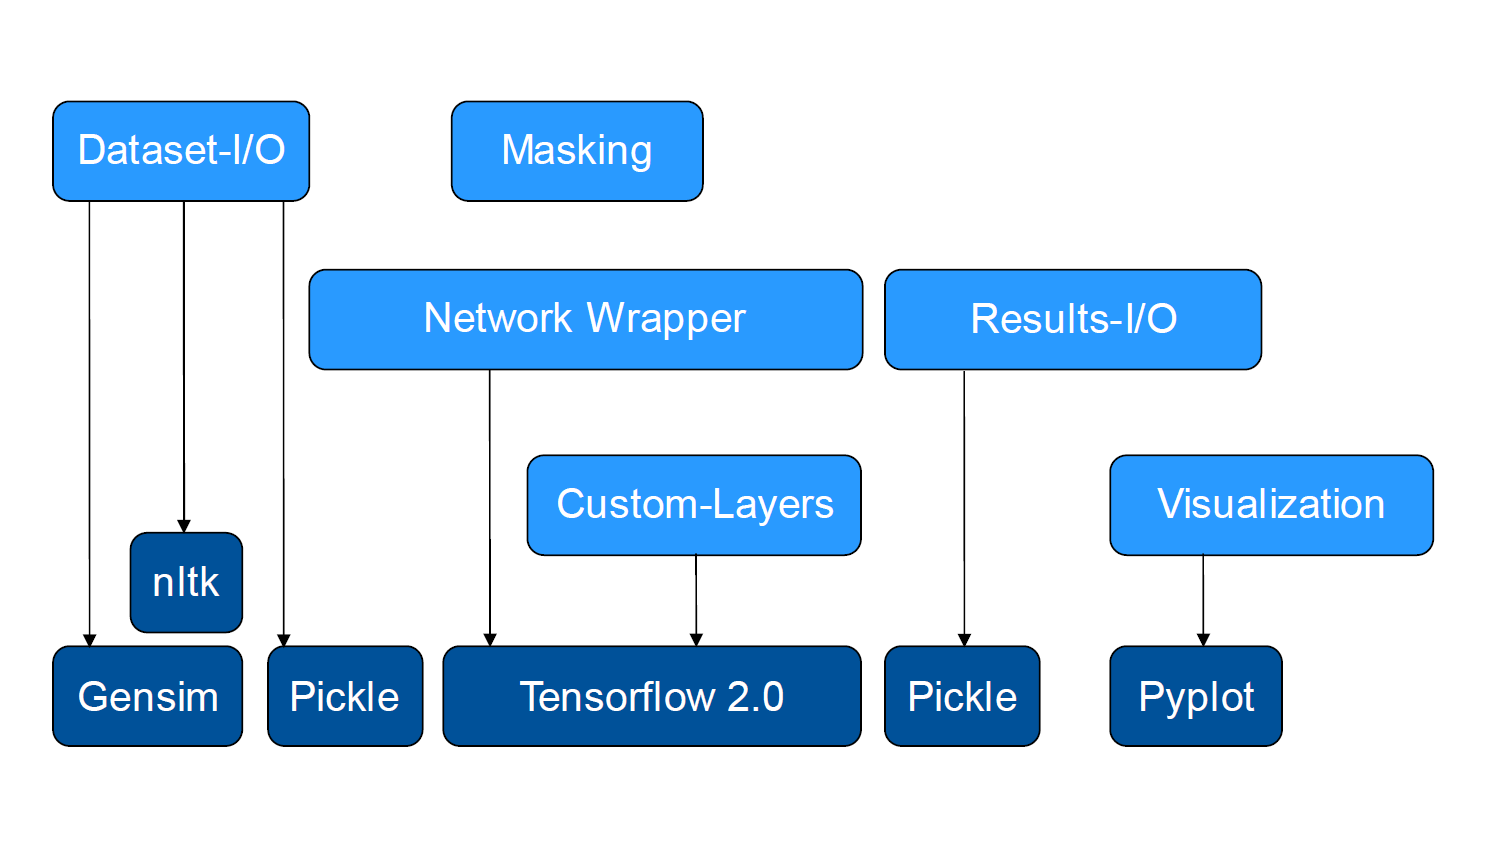
\includegraphics[width=450px]{gfx/structure2.png}
	\caption{project architecture}
	\label{fig:Interaction}
\end{figure}


\section{Summary}